\documentclass{beamer}
\usetheme{Boadilla}
\usepackage{graphicx} % Required for inserting images
\usepackage{amsmath,amssymb}


\DeclareRobustCommand{\bbone}{\text{\usefont{U}{bbold}{m}{n}1}}
\DeclareMathOperator{\EX}{\mathbb{E}}% expected value

\title{Learning "What-if" Explanations For Sequential Decision Making}
\subtitle{IE 708 Project}
\author{Hanish Prashant Dhanwalkar}
% \institute{210100060}
\date{\today}

\begin{document}

\begin{frame}
\titlepage
\end{frame}

\begin{frame}
\frametitle{Batch IRL}
    \textbf{What is IRL:}
    \begin{itemize}
        \item Learning technique that aims to infer the reward function of an agent by observing its behavior in a given environment.
        \item Unlike traditional reinforcement learning, where the reward function is explicitly defined, Batch IRL learns the reward function from a set of expert demonstrations or trajectories.
    \end{itemize}
    
    \textbf{Why Batch IRL}
    \begin{itemize}
        \item \textbf{Online Learning:} Classic IRL algorithms require interactive access to the environment, or full knowledge of the environment’s dynamics.
        \item Limited by the assumption that state dynamics are fully-observable and Markovian. NOT true for domains like medicine, where treatment depends on how patient covariates (tumour, side effects) have evolved over time. 
    \end{itemize}

\end{frame}

\begin{frame}{"What-if" Explanations}
    Incorporating counterfactual reasoning into batch IRL

    \begin{itemize}
        \item Learn a parameterized reward function $R(h_t, a_t)$ that is defined as a weighted sum over potential outcomes for taking action at given history $h_t$.

        \item This helps in reasoning out why an expert (eq. doctor) have chosen a particular action and ``what" would have happen if any other alternative was taken. These experimentation are not possible in medicine domain.
    \end{itemize}
    
\end{frame}

\begin{frame}{Example: Cancer Treatment}
    \begin{itemize}
        \item Consider the decision making process of assigning a binary action given, 
        \begin{itemize}
            \item Tumour volume ($U$)
            \item Side effects ($Z$) 
        \end{itemize}
    
        \item Let $\EX[U_{t+1}[a_t] | h_t]$ and $\EX[Z_{t+1}[a_t] | h_t]$    \\ 
        be the counterfactual outcomes for the two covariates when action $a_t$ is taken given the history $h_t$ of covariates and previous actions.  \\

        \item The reward as the weighted sum of these counterfactuals:
        \begin{itemize}
            \item $R(h_t, a_t) = w_u \EX[U_{t+1}[a_t] | h_t] + w_z \EX[Z_{t+1}[a_t] | h_t]$,
        \end{itemize}  

        \item This allows us to model the preferences of experts: \\
        e.g. finding that $|w_u| > |w_z|$ indicates that the expert is treating more aggressively, by placing more weight on reducing tumour volume than on minimizing side effects.

    \end{itemize}
        
\end{frame}

\begin{frame}{}
    \begin{figure}
        \centering
        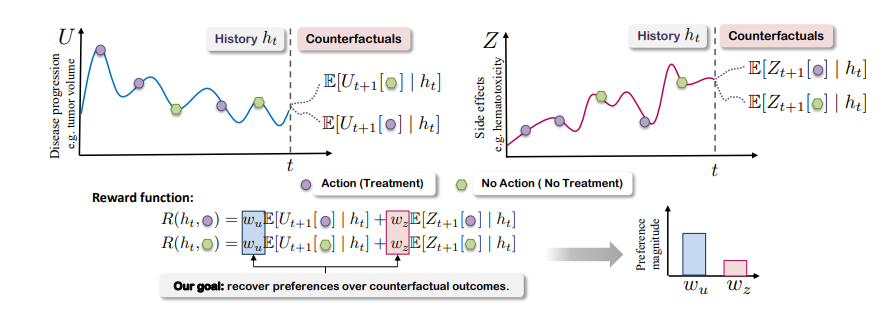
\includegraphics[width=0.9\linewidth]{fig1.png}
        \caption{Explaining decision-making behaviour in terms of preferences over ``what if" outcomes. Evolution of tumour volume ($U$) and side effects ($Z$) under a binary action.}
        \label{fig1}
    \end{figure}
\end{frame}

\begin{frame}{Problem Formulation}
    At timestep $t$, let $X_t \in X$ be the observed patient features and 
    $A_t \in A$ be the action (e.g. treatment) taken.
    Let $x_t$ and $a_t$ be realizations of these random variables, $h_t = (x_0, a_0, . . . , x_{t−1}, a{t−1}, x_t) = (x_{0:t}, a_{0:t−1}) \in H$ be a realization of the history $H_t \in H$ of patient observations and actions.\\
    \begin{itemize}
        \item A policy $\pi : H\times A \xrightarrow{} [0, 1]$, where $\pi(a | h)$ indicates the probability of choosing action $a \in A$ given history $h \in H$ and $\sum_{a \in A}{\pi(a |h)} = 1$.
        \item Taking action $a_t$ under history $h_t$ results in observing $x_{t+1}$ and obtaining $h_{t+1}$. The reward function is $R : H \times A \xrightarrow{} \mathbb{R}$ where $R(h, a)$ represents the reward for taking action a ∈ A given history $h \in H$.
        \item The value function of a policy $\pi$, $V : H \xrightarrow{} \mathbb{R}$ is defined as: $V^{\pi}(h) = \EX[\sum_{t=0}^{\infty} \gamma^tR(H_t, A_t) | \pi, H_0=h]$, where $\gamma \in [0,1)$ is the discount factor.
        \item The action-value function $Q: H \times A \xrightarrow{} \mathbb{R}$ of a policy is defined as $Q^\pi(h,a) = \EX[\sum_{t=0}^{\infty} \gamma^tR(H_t, A_t) | \pi, H_0=h, A_0 = a]$

        
    \end{itemize}
\end{frame}

\begin{frame}{Problem Formulation}
    \begin{itemize}
        
        \item \textbf{Batch IRL}: consider a linear reward function $R(h_t, a_t) = w \cdot \phi(h_t, a_t)$ where $||w||_1 \leq 1$

        \item $\pi_E $ is attempting optimise some unknown reward function $R^*(h_t, a_t) = w^* \cdot \phi(h_t, a_t)$ where $w^*$ are the ‘true’ reward weights.

        \item The value of policy $\pi$ can be re-written as: \\
            \begin{equation*}
                \EX[V^\pi(H_0) = w \cdot \EX[\sum_{t=0}^\infty \gamma^t\phi(H_t, A_t) | \pi]
            \end{equation*}

        \item The feature expectation of $\pi$, defined as the expected discounted cumulative feature vector obtained when choosing actions according to $\pi$ is
            \begin{equation*}
                    \mu^\pi = \EX[\sum_{t=0}^\infty \gamma^t\phi(H_t, A_t) | \pi] \in \mathbb{R}^d 
                \end{equation*}
            such that: $\EX[V^\pi(H_0)] = w \cdot \mu^\pi$
    \end{itemize}
\end{frame}

\begin{frame}{Problem Formulation}
    \begin{itemize}
        \item Our aim is to recover the expert weights $W^*$ as well as find a policy $\pi$ that is close to the policy of the expert $\pi_E$

        \item max-margin IRL approach and measure the similarity between the feature expectations of the expert’s policy and the feature expectations of a candidate policy using $||\mu^{\pi_E}- \mu^\pi||_2$

        \item  In this batch IRL setting, we do not have knowledge of transition dynamics and we cannot sample more trajectories from the environment.
    \end{itemize}
\end{frame}

\begin{frame}{Problem Formulation}
    \begin{itemize}

        \item \textbf{Counterfactual reasoning:} To explain the expert’s behaviour in terms of their trade-off associated with "what if" outcomes

        \item define the feature map $\phi(h_t, a_t)$ part of the reward $R(h_t, a_t) = w \cdot \phi(h_t, a_t)$

        \item Let $Y[a]$ be potential potential outcome, either factual or counterfactual, for treatment $ a \in A$. Using Dataset D, learn feature map $\phi(h_t, a_t)$ such that $\phi(h_t, a_t) = \EX[Y_{t+1}[a_t] | h_t$.
        \item The potential outcomes for the other actions are the counterfactual ones and they allow us to understand what would happen to the patient if they receive a different treatment.
        \item Consider the model for estimating counterfactuals as a black box such that the feature map $\phi$ represents the effect of taking action $a_t$ for history $h_t$.
        \vspace{-0.5cm}
        \begin{equation*}
            R(h_t, a_t) = w \cdot \phi(h_t, a_t) = w \cdot \EX[Y_{t+1}[a_t] | h_t
        \end{equation*}
    \end{itemize}
\end{frame}

\begin{frame}{Batch IRL using Conterfactuals}
    \begin{itemize}
        \item Max-margin IRL starts with an initial random policy $\pi$ and iteratively performs the following steps to recover the expert policy and its reward weighs: 
        \begin{enumerate}
            \item estimate feature expectations $\mu^\pi$ of candidate policy $\pi$,
            \item compute new reward weights $w$,
            \item  find new candidate policy $\pi$ that is optimal for reward function $R$
        \end{enumerate}

        \item This approach finds a policy $\Tilde{\pi}$ that satisfies $||\mu^{\pi_E}- \mu^\pi||_2 < \epsilon$ such that $\Tilde{\pi}$ has an expected value function close the expert policy.

        \item The expert feature expectations can be estimated empirically from the dataset D using:
            \begin{equation*}
                \mu^{\pi_E} = \frac{1}{N} \sum_{i=0}^N \sum_{t=0}^{T^i} \gamma^t \phi(h_t^i, a_t^i)
            \end{equation*}

    \end{itemize}
\end{frame}

\begin{frame}{Batch IRL using Conterfactuals}
    
    \begin{figure}
        \centering
        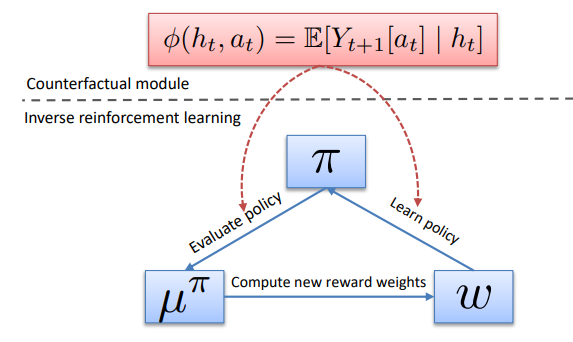
\includegraphics[width=0.7\linewidth]{fig2.png}
        \caption{CIRL. Counterfactuals are used to define $\phi(h, a)$, to estimate feature expectations $\mu^\pi$ of candidate policy $\pi$ in batch setting and to learn optimal policy for reward weights $w$.}
        \label{fig2}
    \end{figure}
\end{frame}

\begin{frame}{Counterfactual $\mu$ - Learning}
    First action a is taken randomly and for $t \geq 1, A_t \sim \pi(\cdot | H_t)$. \\
    This can be re-written as:
    \vspace{-0.3cm}
    \begin{equation*}
        \begin{split}
            \mu^\pi(h,a) & = \phi(h,a) + \EX_{h', a' \sim \pi(\cdot|h')} [\sum_{t=0}^\infty\gamma^t \phi(h_t, a_t) | \pi, H_1 = h', A_1 = a'] \\
             & = \phi(h,a) + \phi\EX_{h', a' \sim \pi(\cdot|h')} [Q^\pi(h', a')]
        \end{split}
    \end{equation*}

    where $h'$ is the next history.

    \begin{itemize}
        \item Existing methods for estimating feature expectations fall into two extremes: \\
        (1) model-based (online)IRL approaches learn a model of the world and then use the model as a simulator to obtain on-policy roll-outs  \\
        (2) batch IRL approaches use Q-learning for off-policy evaluation (Lee et al., 2019), and can only be used to evaluate policies similar to the expert policy and require warm start.
    \end{itemize}
    
\end{frame}

\begin{frame}{Counterfactual $\mu$ - Learning}
    \begin{itemize}
        \item The paper proposes counterfactual $\mu$-learning, a novel method for estimating feature expectations that uses these counterfactuals as part of temporal difference learning with 1-step bootstrapping. 
        \item This approach falls in-between (1) and (2) and allows us to estimate feature expectations for any candidate policy $\pi$ in the batch IRL setting.
        \item The counterfactual $\mu$-learning algorithm learns the $\mu$-values for policy $\pi$ iteratively by updating the current estimates of the $\mu$-values with the feature map plus the $\mu$-values obtained by following policy $\pi$ in the new counterfactual history $h' = (h, a , \EX[Y[a]|h])$
        \begin{equation*}
            \hat{\mu}^\pi \xleftarrow{} \hat{\mu}^\pi(h,a) + \alpha(\phi(h,a) + \gamma \EX_{a' \sim \pi(\cdot|h')}[\hat{\mu}^\pi(h', a')] -  \hat{\mu}^\pi(h', a')
        \end{equation*}
        where $\alpha$ is the learning rate.
    \end{itemize}
    
\end{frame}

\begin{frame}{Batch, Max-Margin CIRL}

    \begin{figure}
        \centering
        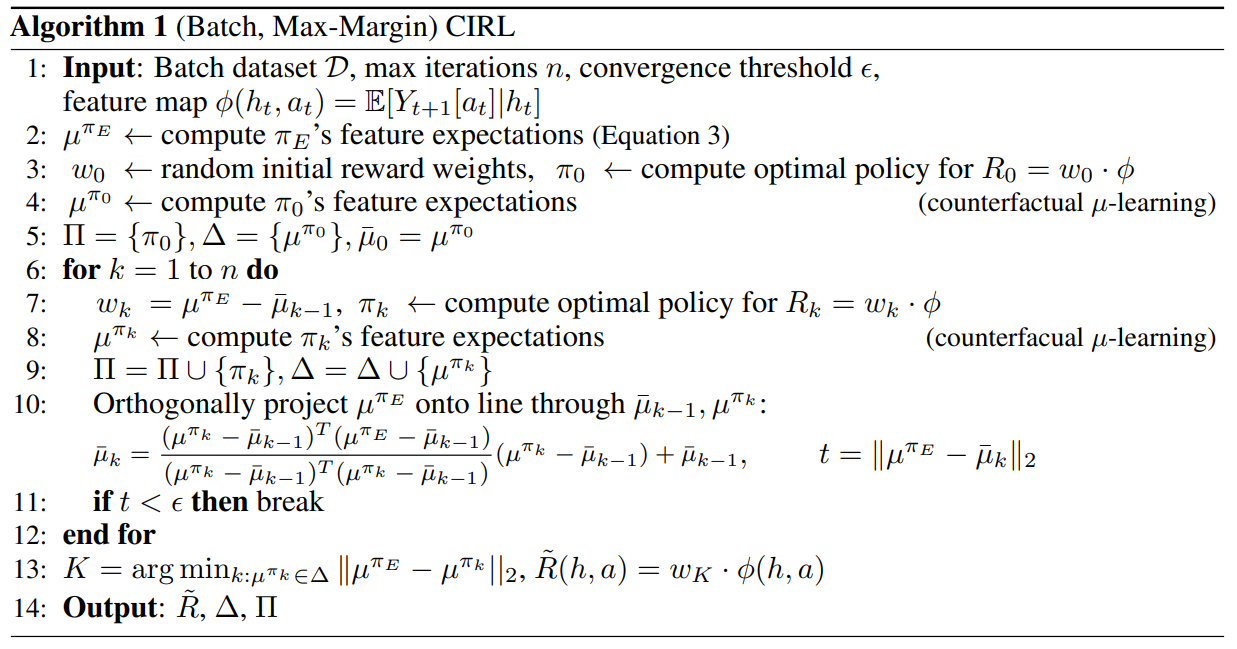
\includegraphics[width=0.9\linewidth]{fig3.png}
        \caption{Psedo Code for CIRL}
        \label{fig3}
    \end{figure}
    
\end{frame}

% \begin{frame}{Advantages of using Counterfactuals and Batch IRL}
%     \begin{itemize}
%         \item Offers a principled approach for parameterizing reward functions in terms of preferences over what-if patient outcomes, which enables us to explain the cost-benefit tradeoffs associated with an expert’s actions.
%         \item by estimating the effects of different actions, counterfactuals readily tackle the off-policy nature of policy evaluation in the batch setting.
        
%     \end{itemize}

%     Thus, Batch IRL with counterfactual reasoning approach can be used in recovering accurate and interpretable descriptions of behavior of experts.
% \end{frame}

\begin{frame}{}
  \centering \Large
  \emph{Thank You}
\end{frame}



\end{document}
